% 黒魔術
\expandafter\ifx\csname ifdraft\endcsname\relax
    \documentclass[a4paper,twoside,12pt,papersize, dvipdfmx]{iirthesis}
    \usepackage{amsmath,amssymb,amsthm}
    \usepackage{graphicx}
    \usepackage{subcaption}
    \usepackage{url}
    \usepackage{otf}
    \usepackage{minitoc}
    \usepackage{bm}
    \usepackage{amsmath,amssymb}
    \usepackage{algorithmic}
    \usepackage{algorithm}
    \begin{document}

    \newcommand{\figref}[1]{\figurename\ref{#1}}
    \newcommand{\tabref}[1]{\tablename\ref{#1}}
    \renewcommand{\eqref}[1]{式~(\ref{#1})}
    \newcommand{\chapref}[1]{\ref{#1}章}
    \newcommand{\secref}[1]{\ref{#1}節}
    \newcommand{\ssecref}[1]{\ref{#1}項}
    \newcommand{\appref}[1]{付録\ref{#1}}
    \newcommand{\algoref}[1]{Algorithm.\ref{#1}}
\fi

\newcommand{\tab}[0]{\;\;\;\;}

\chapter{ハンド動作計画の性能向上と新アルゴリズム}\label{chap::planner}
\minitoc

\section{はじめに}\label{sec::planner::intro}
%ハンドの寸法とかPCの性能の話,閾値,コンフィギュレーションの離散粗さ,動作計画で使ってる情報の説明
本章ではハンドの動作計画における先行研究からの改善点や新たな手法の提案を説明する.本節では,実際の動作計画に使用する設定情報についてまとめる.\par

\paragraph{ハンドの設定}
まずは,ハンドの設定についてである.ハンドは\ssecref{subsec::sicm::oppositehand}の対向型ハンドを以降の全ての動作計画に対して使用している.ハンドの寸法は以下のように設定した(\figref{fig::planner::handsystem}).
\begin{gather}
\notag
\left\{
\begin{aligned}
L &= 60 \mathrm{[mm]} & w& = 35 \mathrm{[mm]} & h &= 415 \mathrm{[mm]}\\
d_0 &= 38 \mathrm{[mm]} & d_1 &= 130 \mathrm{[mm]} & d_2 &= 130 \mathrm{[mm]} & d_3 = 90 \mathrm{[mm]}
\end{aligned}
\right .
\end{gather}


\paragraph{対象物のコンフィギュレーション空間の設定}
対象物コンフィギュレーション空間は$-400 \mathrm{[mm]} \leq x \leq 400 \mathrm{[mm]}$,$-50 \mathrm{[mm]} \leq y \leq 550 \mathrm{[mm]}$,$0 \mathrm{[deg]} \leq \phi \leq 360 \mathrm{[deg]}$の直方体空間と設定した.$(x,y)$の原点は\figref{fig::planner::handsystem}の原点$O$に相当し,$\phi$の原点は以下に記す対象物の姿勢$0^\circ$に相当する.前述の通り,コンフィギュレーション空間は格子状に分割し,離散的に取り扱っている.この格子点幅は$(\Delta x, \Delta y, \Delta \phi) = (10 \mathrm{[mm]}, 10 \mathrm{[mm]}, 5 \mathrm{[deg]})$と設定した.$P_{\mathrm {far}}$は,$\mathcal{C}_{\mathrm{free\_ICS}}$の導出で用いる,ハンドから十分に離れた点群であり,以下の式で表される点群と設定した.なお,$C_{\mathrm {space}}$はコンフィギュレーション空間の全離散点群を表す.
\begin{gather}
\notag
P_{\mathrm {far}} = \{ (x, y, \phi) \in C_{\mathrm {space}} \,|\, x = -400 \mathrm{[mm]} \lor x = 400 \mathrm{[mm]} \lor y = 550\mathrm{[mm]} \}
\end{gather}

\paragraph{対象物の形状情報}
本論文では,長方形物体,三角形物体,L字型物体,T字型物体を対象に動作計画を行った.これらの対象物の寸法情報や姿勢の定義について述べる.長方形物体は\figref{}のように設定した.図心は対角線の交点であり,姿勢は短辺が水平方向となるように置いた状態を$0^\circ$とした傾き角度となる.三角形物体は\figref{}のように設定した.図心は外接円の中心であり,姿勢は$e_1$が水平方向となるように置いた状態を$0^\circ$とした傾き角度である.そのため,ユーザは三角形物体の形状情報を設定するとき,どの辺が$e_1$かを把握し,そのうえで目標姿勢を与える必要がある.L字型物体は\figref{}のように設定した.図心は\figref{}のように補助線を引いて得られる長方形の対角線交点である.姿勢は文字「L」を$0^\circ$とした傾き角度である.T字型物体は\figref{}のように設定した.図心,姿勢ともにL字型と同様である.なお,傾きは$0 \mathrm{[deg]} \leq \phi \leq 360 \mathrm{[deg]}$で表し,時計回りに測る.

\paragraph{PCのスペック}
OS:Ubuntu 22.04.1 LTS,CPU:AMD Ryzen 7 3700X 8-Core Processor,クロック周波数:4.43[GHz],RAM:32.0[GB]のPCで計算する.

%\begin{figure}[b]
%\centering
%\includegraphics
%\caption{ハンドの図,写真じゃなくてパワポとかで}
%\label{fig::planner::handsystem}
%\end{figure}

\section{順探索アルゴリズム}\label{sec::planner::straight}
改めて\chapref{chap::sicm}のハンド動作計画の流れを振り返る.まず,入力はハンドの初期姿勢と対象物の形状情報,そして対象物の目標位置・姿勢である.これらを基に,ハンド初期姿勢からRRTによりランダムにサンプリングし,その都度対象物の形状情報から$\mathcal{C}_{\mathrm{free\_obj}}$を計算する.ケージング成立条件,ケージングマニピュレーション可能条件の満足を確認しつつ探索を進め,対象物の目標位置・姿勢から決まる探索終了条件を満たせば動作計画が完了する.出力としては,ハンドの関節角度の時系列データが得られる.\par
この動作計画アルゴリズムを順探索アルゴリズムと呼ぶこととする.この順探索アルゴリズムには,計算時間が遅い,位置決め精度が悪いという2つの課題がある.以下の項は,これらの解決方法についてであり,前者の課題に対しては,\ssecref{subsec::planner::goalcond},\ssecref{subsec::planner::dfs}で,後者の課題に対しては,\ssecref{subsec::planner::formclosure}で説明する.

\subsection{探索終了条件の緩和}\label{subsec::planner::goalcond}
\secref{sec::sicm::planning}の通り,先行研究では対象物の目標位置・姿勢として$P_G (x_{\mathrm {goal}}, y_{\mathrm {goal}}, \phi_{\mathrm {goal}})$のコンフィギュレーション空間の1点を指定していた.しかし,本手法はパーツフィーダへの応用を想定しており,この際対象物を整列後,ベルトコンベアに乗せて生産ライン方向である$x$方向へ流す.そのため,$x$方向への目標設定は必須ではない.そこで,対象物の目標位置・姿勢を$P_G (x_{\mathrm {any}}, y_{\mathrm {goal}}, \phi_{\mathrm {goal}})$と$y$,$\phi$のみを指定するようにした.\par
これに従って,収束度$e$の定義を\eqref{eq::planner::e},探索終了条件を\eqref{eq::planner::goalcondition}のように変更した.
\begin{gather}
e = \max \sqrt{(w_1\Delta x)^2 + (w_2(y-y_{\mathrm{goal}}))^2 + (w_3(\phi-\phi_{\mathrm{goal}}))^2} \label{eq::planner::e} \\
e \leq \varepsilon \label{eq::planner::goalcondition} \\
\because  \Delta x = \dfrac{\max x  - \min x}{2} ,\;\; (x, y, \phi) \in \mathcal{C}_{\mathrm{free\_obj}} \notag
\end{gather}
これにより,$x$方向に関しては座標の調整が必要なくなったため,先行研究より早い探索終了が見込める.

\subsubsection{計算時間の比較}
\eqref{eq::planner::e}の収束度$e$の定数$w_1$,$w_2$,$w_3$を次のように設定した.
\begin{gather}
\notag
w_1=1 \mathrm{[mm^{-1}]} \tab w_2=1 \mathrm{[mm^{-1}]} \tab w_3=1 \mathrm{[deg^{-1}]}
\end{gather}
以降の収束度$e$の計算にもこれらの値を用いる.


\subsection{$\mathcal{C}_{\mathrm{free\_obj}}$の効率的な抽出}\label{subsec::planner::dfs}
\cite{komiyama2021}では$\mathcal{C}_{\mathrm{free\_obj}}$の抽出にあたって以下のような方法が取られていた.
\begin{enumerate}
\item 対象物のコンフィギュレーション空間の離散点群を全走査し,$\mathcal{C}_{\mathrm{free}}$を取り出す \label{planner::fullscan}
\item DBSCAN法\cite{}により隣り合う周囲26点群を同クラスタとするクラスタリングを$\mathcal{C}_{\mathrm{free}}$に対して行う\label{planner::clustering}
\item 手順\ref{planner::clustering}のクラスタを$\mathcal{C}_{\mathrm{free\_ICS}}$と$\mathcal{C}_{\mathrm{free\_ECS}}$に分ける
\item $\mathcal{C}_{\mathrm{free\_ICS}}$の内,\eqref{eq::sicm::continuous}に基づいて$\mathcal{C}_{\mathrm{free\_obj}}$を抽出する
\end{enumerate}
対象物のコンフィギュレーション空間の離散粗さを\secref{sec::planner::intro}のように設定した場合,点群数は約33万個となる.手順\ref{planner::fullscan}では,この点群を全走査するため計算時間が長くかかり,ボトルネックとなっている.\par

そこで,\eqref{eq::sicm::continuous}の直前$(t-\Delta t)$のハンド姿勢における$\mathcal{C}_{\mathrm{free\_obj}}(t-\Delta t)$と現在$(t)$のハンド姿勢における$\mathcal{C}_{\mathrm{free\_obj}}(t)$はオーバーラップしているという性質を応用して,$\mathcal{C}_{\mathrm{free\_obj}}(t-\Delta t)$を起点として,オーバーラップしている$\mathcal{C}_{\mathrm{free\_ICS}}$を探すという手法を提案する.\par

まず,$\mathcal{C}_{\mathrm{free\_obj}}(t-\Delta t)$の任意の一点を取り出す.壁やロボットハンドとの干渉がないか確認し,干渉があった場合は別の点を取り出す.この点を起点として,周囲を探索する.このとき,\figref{}のように周囲の26個の方向に番号を付け,\figref{}のような木構造を作成する.この木構造は,根が取り出した起点であり,葉が起点周囲の点群となっており,周囲の探索手順の全組み合わせを表している.例えば根から1,6,13と進んだ場合は,起点から1の方向の点へ移動し,そこから6の方向へ進み,さらに13の方向へ3ステップ進んだ点へ到達していることを表す.\par

この木構造を用いて,「深さ優先」のアプローチで探索を行う.
もし,探索が無限遠点$P_{\mathrm {far}}$へ到達した場合,つまり探索中の領域が$\mathcal{C}_{\mathrm{free\_ECS}}$であった場合,その領域は破棄することとなる.無駄な探索を増やさないため,その領域が$P_{\mathrm {far}}$へ到達するかどうかはなるべく早く判断したい.幅優先探索のようなアプローチを取ると,起点から全方向へ同じペースで探索が進むため,$P_{\mathrm {far}}$への到達が遅くなり,無駄な探索が多くなる.そこで,深さ優先探索というアプローチを取ると,任意の方向へ一直線に進めるだけ進むため,早い段階で$P_{\mathrm {far}}$へ到達することができる.\par

$\mathcal{C}_{\mathrm{free\_obj}}(t-\Delta t)$の内,探索されていない点がある場合はその点を起点として上記の操作を繰り返す.$P_{\mathrm {far}}$へ到達しなかった領域が$\mathcal{C}_{\mathrm{free\_obj}}(t)$となる.以上のアルゴリズムをより具体的にまとめたものを\algoref{algo::planner::dfs}に示す.


\subsubsection{計算時間の比較}


\subsection{位置決め精度向上アルゴリズム}{\label{subsec::planner::formclosure}
計算時間の観点から,収束度$\varepsilon$は広めに設定したい.そのため,動作計画で得られたハンド最終姿勢では対象物の位置・姿勢決め精度は十分ではない.そこで,以降に示す方法によって動作計画で得られたハンド最終姿勢から微調整を加え,位置決め精度の向上を試みた.
\subsubsection{アルゴリズム}
本アルゴリズムでは,動作計画により得られた最終姿勢から更に狭まる方向へ,更にケージングが強まる方向へ微調整する.そのため,この微調整中はケージング成立条件,ケージングマニピュレーション可能条件の両者が成立していると考え,本アルゴリズムではこれを前提としている.以下,具体的なアルゴリズムについて述べる.\par
まず,対象物を目標位置・姿勢$P_G (x_{\mathrm m}, y_G, \theta_G)$に仮想的に配置する.ここで,目標位置・姿勢の$x$座標に関して,\secref{subsec::planner::goalcond}の方法により,動作計画毎に位置決めされる対象物の$x$位置は変わる.そこで,$x_{\mathrm m}$には各々$\mathcal{C}_{\mathrm{free\_obj}}$の任意の$x$座標値を設定することとする.次に,片ハンドずつ対象物への距離を詰めていく.具体的には,ハンドの根元側の関節から手先側の関節の順で狭めていき,各々いずれかのハンドが対象物や他方ハンドと接触する直前で止める.この操作により,対象物の動ける範囲はさらに縮小され,位置・姿勢決め精度が向上する.\par
上記の片ハンドずつ対象物への距離を詰めていくという部分に関して,本アルゴリズムでは,左ハンド,右ハンドの順で狭めるパターンと右ハンド,左ハンドの順で狭めるパターンの2パターンを試みる.そして,より位置・姿勢決め精度が向上した方を最終的なハンド姿勢として採用する.

\subsubsection{結果}
本アルゴリズムを用いて,どの程度位置決め精度が向上するかを評価する.評価には\eqref{eq::planner::e}の収束度$e$を用い,小さいほどゴールへの収束度が高く,位置・姿勢決め精度が向上したと判断する.
figref{fig::afterfc}のように,$\varepsilon$の値はアルゴリズム適用前が48.8だったのに対し,右ハンド,左ハンドの順の場合は25.5で,左ハンド,右ハンドの順で狭める場合は19.6となった.これらより,位置・姿勢決め精度の向上を確認できた.
また,上記の2パターンの狭め方を試したことに関して,多くは同じ結果が得られるが,今回の場合のように精度に差が出る場合があることがあり,複数パターンを試すことの有効性が確認できた.今後,他の狭め方もパターンに含めることで更なる精度向上が望める可能性がある. \par
課題点としては,今回用いたハンドの関節角上限が$90^{\circ}$であるため,\figref{fig::afterfc}の左ハンドの手先リンクのように,対象物まで狭めきれない場合がある.実機を改良して$90^{\circ}$以上回転を可能にすることで,更なる精度向上が望める.
\begin{figure}[b]
\centering
\begin{minipage}{0.33\hsize}
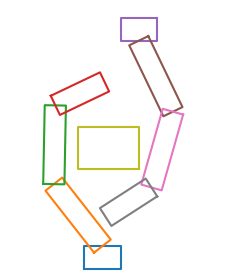
\includegraphics[width=0.9\hsize]{fig/3-new-planner/rec_before_FC.png}
\subcaption{Before applying}\label{fig::planner::beforefc}
\end{minipage}\hfill
\begin{minipage}{0.33\hsize}
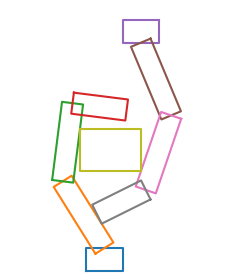
\includegraphics[width=0.9\hsize]{fig/3-new-planner/rec_FC_left_right.png}
\subcaption{left$\rightarrow$right}\label{fig::planner::afterfclr}
\end{minipage}\hfill
\begin{minipage}{0.33\hsize}
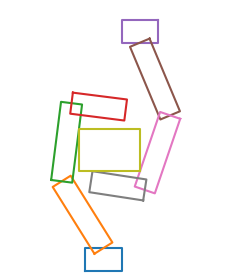
\includegraphics[width=0.9\hsize]{fig/3-new-planner/rec_FC_right_left.png}
\subcaption{right$\rightarrow$left}\label{fig::planner::afterfcrl}
\end{minipage}
\end{figure}

\section{逆探索アルゴリズム}\label{sec::planner::reverse}
\subsection{RRTを用いた逆探索アルゴリズム}
\secref{sec::planner::straight}の順探索では,任意の初期姿勢から対象物の目標位置・姿勢座標$P_G$を目指している.しかし,RRTはランダムサンプリングであるため$P_G$から遠ざかるような方向へも探索が進むという点で効率が悪い.そこで,対象物が目標位置・姿勢で位置決めされた時のハンド姿勢$\bm{\theta_G}$を探索の開始点とし,マニピュレーションの初期状態へと遡る方向へ探索する.つまり,RRTを用いて,$t=T (任意)$から$t=0$へ向けて探索を行う.これを以下では逆探索アルゴリズムと呼ぶ.

\subsubsection{探索終了条件}
逆探索であるため,探索の終了状態はマニピュレーションの初期状態に相当する.マニピュレーションの初期状態に求められることとしては,なるべく多様な対象物位置・姿勢を取り扱えるということが挙げられる.そこで,探索の終了条件を,物体が取りうる姿勢群を表す$C_{\mathrm{free\_obj}}$が閾値以上になった時と定めた.\par
このように,逆探索アルゴリズムでは探索の終了条件に座標の指定がなく,ただ$C_{\mathrm{free\_obj}}$の領域を広げればよい.そのため,順探索のような無駄な探索方向が少なくっており,探索効率の改善が見込める.

\subsubsection{ケージングマニピュレーション可能条件}\label{subsec::planner::revcm}
条件自体は,\secref{sec::sicm::caging}と変わらず,時間$t-\Delta t$における物体の存在領域$\mathcal{C}_{\mathrm{free\_obj}}(t-\Delta t)$に対する時間$t$の$C_{\mathrm{free\_obj}}(t)$がただ一つ存在する場合に成立と判定される.しかし,時間が逆行した方向への探索であるため処理が異なる.処理は\figref{fig::planner::cm}のような3パターンに大別できる.ただし,実際の$\mathcal{C}_{\mathrm{free\_obj}}$領域は3次元であるが,\figref{fig::planner::cm}では簡単のため2次元としてモデル化している.\figref{fig::planner::cm1}は$C_{\mathrm{free\_obj}}(t)$に対してオーバーラップしている$C_{\mathrm{free\_obj}}(t-\Delta t)$が複数ある場合である.これは,各々の$C_{\mathrm{free\_obj}}(t-\Delta t)$から見るとオーバーラップしている$C_{\mathrm{free\_obj}}(t)$は1つのみであるため,ケージングマニピュレーション可能条件を満たしている.この判定は,逆探索アルゴリズムでは$C_{\mathrm{free\_obj}}$が複数個存在しうることを意味している.すなわち,\figref{fig::planner::cm2}の状況も発生しうる.これは,$C_{\mathrm{free\_obj}}(t-\Delta t)$に対してオーバーラップしている$C_{\mathrm{free\_obj}}(t)$が複数あるので,ケージングマニピュレーション可能条件を満たしていない.\figref{fig::planner::cm3}では,そもそもオーバーラップがないので不成立である.以上の3つで全ての場合に対して判定することができる.

%\begin{figure}[b]
%\begin{minipage}{0.33\hsize}
%\includegraphics[width=0.95\hsize]{fig/}
%\subcaption{}\label{fig::planner::cm1}
%\end{minipage}\hfill
%\begin{minipage}{0.33\hsize}
%\includegraphics[width=0.95\hsize]{fig/}
%\subcaption{}\label{fig::planner::cm2}
%\end{minipage}\hfill
%\begin{minipage}{0.33\hsize}
%\includegraphics[width=0.95\hsize]{fig/}
%\subcaption{}\label{fig::planner::cm3}
%\end{minipage}
%\caption{The patterns of the condition for caging manipulability for reverse exploring}
%\label{fig::planner::cm}
%\end{figure}

\subsubsection{逆探索アルゴリズムにおける$C_{\mathrm{free\_obj}}$の抽出}
逆探索アルゴリズムの$C_{\mathrm{free\_obj}}$抽出も\ssecref{subsec::planner::dfs}の考え方を基に実装する.まず,$t+\Delta t$における$C_{\mathrm{free\_obj}}(t+\Delta t)$の任意の点を起点として,深さ優先探索で$C_{\mathrm{free\_obj}}(t)$を抽出する.次に,$C_{\mathrm{free\_obj}}(t+\Delta t)$と$C_{\mathrm{free\_obj}}(t)$のオーバーラップを前項を基に考える.ここで,本実装では\ssecref{subsec::planner::dfs}の方法により,$C_{\mathrm{free\_obj}}$のみを抽出するようにしている.しかし通常,$C_{\mathrm{free\_obj}}$の周囲には別領域の$C_{\mathrm{free\_ICS}}$が存在している.したがって,$C_{\mathrm{free\_obj}}(t)$と$C_{\mathrm{free\_ICS}}(t+\Delta t)\, \ni C_{\mathrm{free\_obj}}(t+\Delta t)$のオーバーラップを考える必要がある.\par
そこで,$C_{\mathrm{free\_obj}}(t)$を起点として,再度$t+\Delta t$のハンド姿勢に対して深さ優先探索で$C'_{\mathrm{free\_obj}}(t+\Delta t)$を抽出する.この$C'_{\mathrm{free\_obj}}(t+\Delta t)$の領域が0個もしくは複数個ある場合,ケージングマニピュレーション可能条件を満たさないので,$C_{\mathrm{free\_obj}}(t)$は妥当ではないと判定する.以上の処理を\algoref{algo::revdfs}にまとめる.


\subsection{位置決め最適姿勢生成アルゴリズム}
\subsection{計算時間の比較}


\section{両側探索アルゴリズム}\label{sec::planner::connect}
\secref{sec::planner::reverse}の逆探索アルゴリズムでは,期待したほどの計算時間の向上は得られなかった.そこで,順探索アルゴリズムと逆探索アルゴリズムを組み合わせた両探索アルゴリズムを提案する.
\subsection{RRT-Connectを用いた両側探索アルゴリズム}
RRT-Connect\cite{kuffner2000}を用いて両側探索アルゴリズムを構築する.これは,順探索アルゴリズムにおける探索初期状態$\bm {\theta}_S$と逆探索アルゴリズムにおける探索初期状態$\bm {\theta}_G$から交互に枝を伸ばしていき,これらの枝が連結した時,その連結経路を解として探索を終了するアルゴリズムである.なお,本アルゴリズムでは順探索アルゴリズム,逆探索アルゴリズムの探索終了条件も残しており,合計3つの探索終了条件の内,いずれかを満たせば終了するようになっている.具体的なアルゴリズムは以下のようになっている(\figref{}).
\begin{enumerate}
\item 順探索におけるハンドの初期ノード(姿勢)$\bm{q}_{\mathrm init}$と逆探索におけるハンドの初期ノード$\bm{q}_{\mathrm goal}$を設定する.以降,$\bm{q}_{\mathrm init}$を起点としたグラフを$T_{\mathrm forward}$,$\bm{q}_{\mathrm goal}$を起点としたグラフを$T_{\mathrm reverse}$とする
\item ハンドの任意のノード$\bm{q}_{\mathrm sample}$をサンプリングし,$T_{\mathrm forward}$の内,$\bm{q}_{\mathrm{sample}}$から最も近いノード$\bm{q}_{\mathrm{nearest}}$を見つける\label{algo::planner::sampling}
\item $\bm{q}_{\mathrm{nearest}}$から$\bm{q}_{\mathrm{sample}}$の方向へ長さ$\Delta l$の枝を伸ばし,そのノードを$\bm{q}_{\mathrm{new}}$とする
\item $\bm{q}_{\mathrm{new}}$において環境とハンドまたはハンド同士の干渉,ケージングに関する2条件を判定し,妥当でなければ手順\ref{algo::planner::sampling}に戻る
\item $\bm{q}_{\mathrm{new}}$と一番近いノード$\bm{q}_{\mathrm{opposite\_near}}$を$T_{\mathrm reverse}$から探索する\label{algo::planner::biasbegin}
\item $\bm{q}_{\mathrm{opposite\_near}}$から$\bm{q}_{\mathrm{new}}$に向けて長さ$\Delta l$の枝を伸ばし,$\bm{q}_{\mathrm{opposite\_new}}$とする\label{algo::planner::proceed}
\item $\bm{q}_{\mathrm{opposite\_new}}$において環境とハンドまたはハンド同士の干渉,ケージングに関する2条件を判定する
\item $\bm{q}_{\mathrm{opposite\_new}}$が妥当かつ探索終了条件を満たさない場合,$\bm{q}_{\mathrm{opposite\_new}}$を$\bm{q}_{\mathrm{opposite\_near}}$とし,手順\ref{algo::planner::proceed}に戻る\label{algo::planner::biasend}
\item $\bm{q}_{\mathrm{opposite\_new}}$が妥当でない場合,役割を入れ替えて(kwsk)手順\ref{algo::planner::sampling}に戻る
\item $\bm{q}_{\mathrm{opposite\_new}}$が探索終了条件を満たせば終了\label{algo::planner::goalcond}
\end{enumerate}

本アルゴリズムの特徴は二つある.一つ目は,探索終了条件を3つ設定していることである.それぞれ,$T_{\mathrm forward}$が順探索アルゴリズムの探索終了条件を満たす,$T_{\mathrm reverse}$が逆探索アルゴリズムの探索終了条件を満たす,$T_{\mathrm forward}$と$T_{\mathrm reverse}$が繋がり,結合点間のケージング2条件も満たす,の3つとなっている.いずれかを満たせばよいため,順探索アルゴリズム,逆探索アルゴリズムと比べて条件は緩くなっていると言える.二つ目は,手順\ref{algo::planner::biasbegin}から\ref{algo::planner::biasend}にかけて非常に強いバイアスがかかるという点である.スタートからゴール方向へ,ゴールからスタート方向へ進めるだけ進めるというバイアスがかかっているため,順探索アルゴリズムや逆探索アルゴリズムのようなランダムサンプリングに比べて効率的な探索になっている.これら二つの特徴から計算時間の短縮が見込める.

\subsection{計算時間の比較}

% 白魔術
\expandafter\ifx\csname ifdraft\endcsname\relax
    \end{document}
\fi
